\chapter{Ergebnisanalyse}

\todo{nochmal schauen ob Überleitung noch stimmt wenn Implementierungsteil geschriebten wurde...}
Nachdem im letzten Abschnitt ausführlich beschrieben wurde wie der komplette Komponentenstack im Detail implementiert wurde, werden im Folgenden auf die erhaltenen Metriken erläutert. Es wird insbesondere auf die Bedeutung einzelner Messwerte, sowie die auf mögliche Begründungen dieser eingangen.


\todo{folgende Stichpunkte entfernen}
\begin{itemize}
  \item Latenzzeit im Durchschnitt sowie als zeitliche Historie
  \begin{itemize}
    \item Abschnitt \emph{vor} Datenaufnahme gesondert betrachten
    \item Abschnitt \emph{nach} Datenaufnahme gesondert betrachten
    \item Gesamte Pipeline betrachten
  \end{itemize}
  \item Skalierungsdauer jeweils pro verwendeter Backend-Technologie festzuhalten
  \begin{itemize}
    \item Skalierung anhand eingehender Nachrichten mittels Stufenmodell
    \item Skalierung mittels direkter Benutzeranfrage (ohne eingehende Nachrichten)
    \item Metriken als Datensätze in einer Datenbank hinterlegt
    \item Durchschnittliche Startzeit pro Containeranzahl 
    \item Durchschnittliche Startzeit pro Skalierungsstufe 
    \item Gesamtdurchschnittliche Startzeit als einzelner Messwert
    \item Metriken als zeitlicher visualisiert
  \end{itemize}
\end{itemize}




\section{Ergebnisse}
\begin{itemize}
  \item Vorstellung der erhaltenen Daten
  \item Interpretation / Analyse allerdings Teil vom naechsten Kapitel?
\end{itemize}

\subsection{Latenzzeit}


\begin{tikzpicture}
  \begin{axis}[xlabel={Zusätzlich hochgefahrende Container}, ylabel={Startzeit}]
    \addplot table [x=additionalCnt, y=startupTime, col sep=comma] {kapitel/ergebnisanalyse/_data/springSpecificBenchmarks.csv};
    \addlegendentry{Spring Boot}
    \addplot table [x=additionalCnt, y=startupTime, col sep=comma] {kapitel/ergebnisanalyse/_data/nodeSpecificBenchmarks.csv};
    \addlegendentry{Node.js}
  \end{axis}
\end{tikzpicture}

\begin{tikzpicture}
  \begin{axis}[xlabel={Zusätzlich hochgefahrende Containerrrrr}, ylabel={Startzeit}]
    \addplot table [xbar, x=additionalCnt, y=startupTime, col sep=comma] {kapitel/ergebnisanalyse/_data/springSpecificBenchmarks.csv};
    \addlegendentry{Spring Boot}
    \addplot table [x=additionalCnt, y=startupTime, col sep=comma] {kapitel/ergebnisanalyse/_data/nodeSpecificBenchmarks.csv};
    \addlegendentry{Node.js}
  \end{axis}
\end{tikzpicture}

% \begin{tikzpicture}
 
  % \begin{axis} [xbar]
  % \addplot coordinates {
  %     (Nodejs,6610) 
  %     (Spring,35336)
  % };
  % \end{axis}
   
  % \end{tikzpicture}

% \begin{table}[ht]
%   \caption{Partial horizontal line}
%   \begin{tabular}{lll}
%       \hline
%       \multicolumn{2}{c}{Multi-column}&234234\\
%       \cline{1-2}
%       &Nachrichteneingang&213123\\
%       &Verarbeitungsdauer&324324\\
%       \hline
%   \end{tabular}
%   % \end{center}
%   \label{tab:multicol}
%   \end{table}

\begin{tabular}{@{}lc@{}}
  \toprule
  Metrik & Dauer \\
  \midrule
  Node.js \\
  \hspace{3mm}Gesamtdurchschnitt & 12312 \\
  \hspace{3mm}Nachrichteneingang & 12312 \\
  \hspace{3mm}Verarbeitungsdauer & 12312 \\
  \midrule
  Spring Boot \\
  \hspace{3mm}Gesamtdurchschnitt & 12312 \\
  \hspace{3mm}Nachrichteneingang & 12312 \\
  \hspace{3mm}Verarbeitungsdauer & 12312 \\
  \bottomrule
  \end{tabular}

\begin{figure}
	\centering
	\caption[Startzeit Services]{Durchschnittliche Startzeit pro Service}
  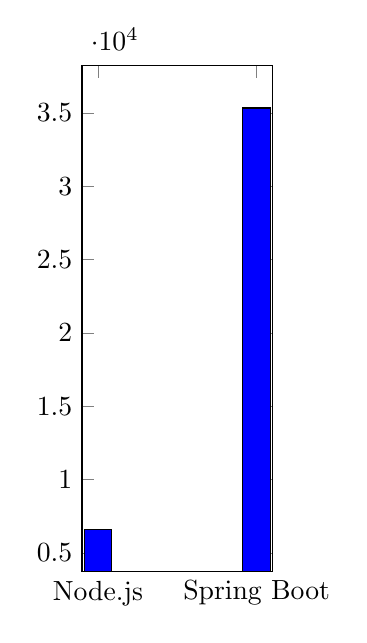
\begin{tikzpicture}
    \begin{axis}[
        symbolic x coords={Node.js,Spring Boot},
        width=4cm,
        height=8cm,
        xtick=data]
        \addplot[ybar,fill=blue] coordinates {
            (Node.js,6610)
            (Spring Boot,35336)
        };
    \end{axis}
  \end{tikzpicture}
\end{figure}

\begin{figure}
	\centering
	\caption[Startzeit Stufenübersicht]{Durchschnittliche Startzeit stufenweise - Node}
  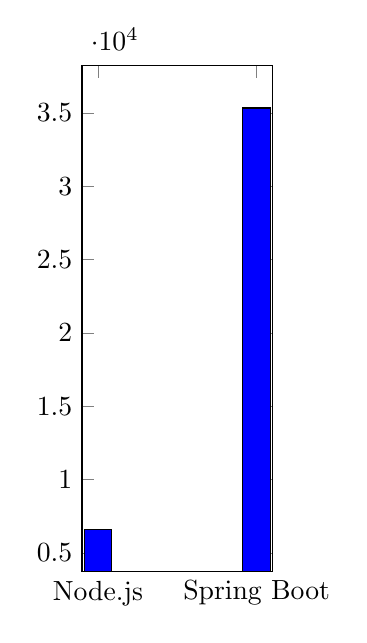
\begin{tikzpicture}
    \begin{axis}[
        symbolic x coords={Node.js,Spring Boot},
        width=4cm,
        height=8cm,
        xtick=data]
        \addplot[ybar,fill=blue] coordinates {
            (Node.js,6610)
            (Spring Boot,35336)
        };
    \end{axis}
  \end{tikzpicture}
\end{figure}




% \begin{tikzpicture}
%   \begin{axis}[
%       coords={Nodejs, Spring Boot},
%       xtick=data,
%       width=3cm,
%       height=5cm
%     ]
%       \addplot[ybar,fill=blue] coordinates {
%           (Nodejs,      6610)
%           (Spring Boot,  35336)
%       };
%   \end{axis}
% \end{tikzpicture}

% \begin{figure}
%   \begin{tikzpicture}
%     \begin{axis}[
%       mbarplot,
%       ymin = 0,
%       ymax = 1,
%       xlabel={},
%       ylabel={},
%       width=0.9\textwidth,
%       height=7cm,
%       xtick=data,
%       symbolic x coords={KNN,E1,E2,E3,E4}
%     ]
%       \addplot table [x=serviceName, y=averageStartupTime, col sep=comma] {kapitel/ergebnisanalyse/_data/nodeSpecificBenchmarks.csv};
%       \legend{Service Startzeit - Durchschnitt}

%     \end{axis}
%   \end{tikzpicture}
% \end{figure}


\subsection{Skalierungsdauer}




\section{Analyse}
\begin{itemize}
  \item Interpretation / Analyse der Daten
  \item Begruendung fuer Verhalten suchen
\end{itemize}

\section{Diskussion}

\subsection{Begr\"undung Startupzeit}
\begin{itemize}
  \item Warum Node.js schneller ist
\end{itemize}

\begin{itemize}
  \item Erlaeutern warum die erhaltenen Ergebnisse in einem real-life Szenario vielleicht nicht aussagekraeftig sein koennten
\end{itemize}
